\section{System}\label{sec:System}
\todo[inline, color=red]{Vera}

\subsection{Lighting Model}\label{sec:lightingmodel}
\todo[inline, color=red]{Vera}

\subsection{Contours}\label{sec:contours}
\todo[inline, color=red]{Vera}
\subsubsection{Find Contours}\label{sec:findContours}
\todo[inline, color=red]{Vera}
\begin{figure}[H] 
	\center 
	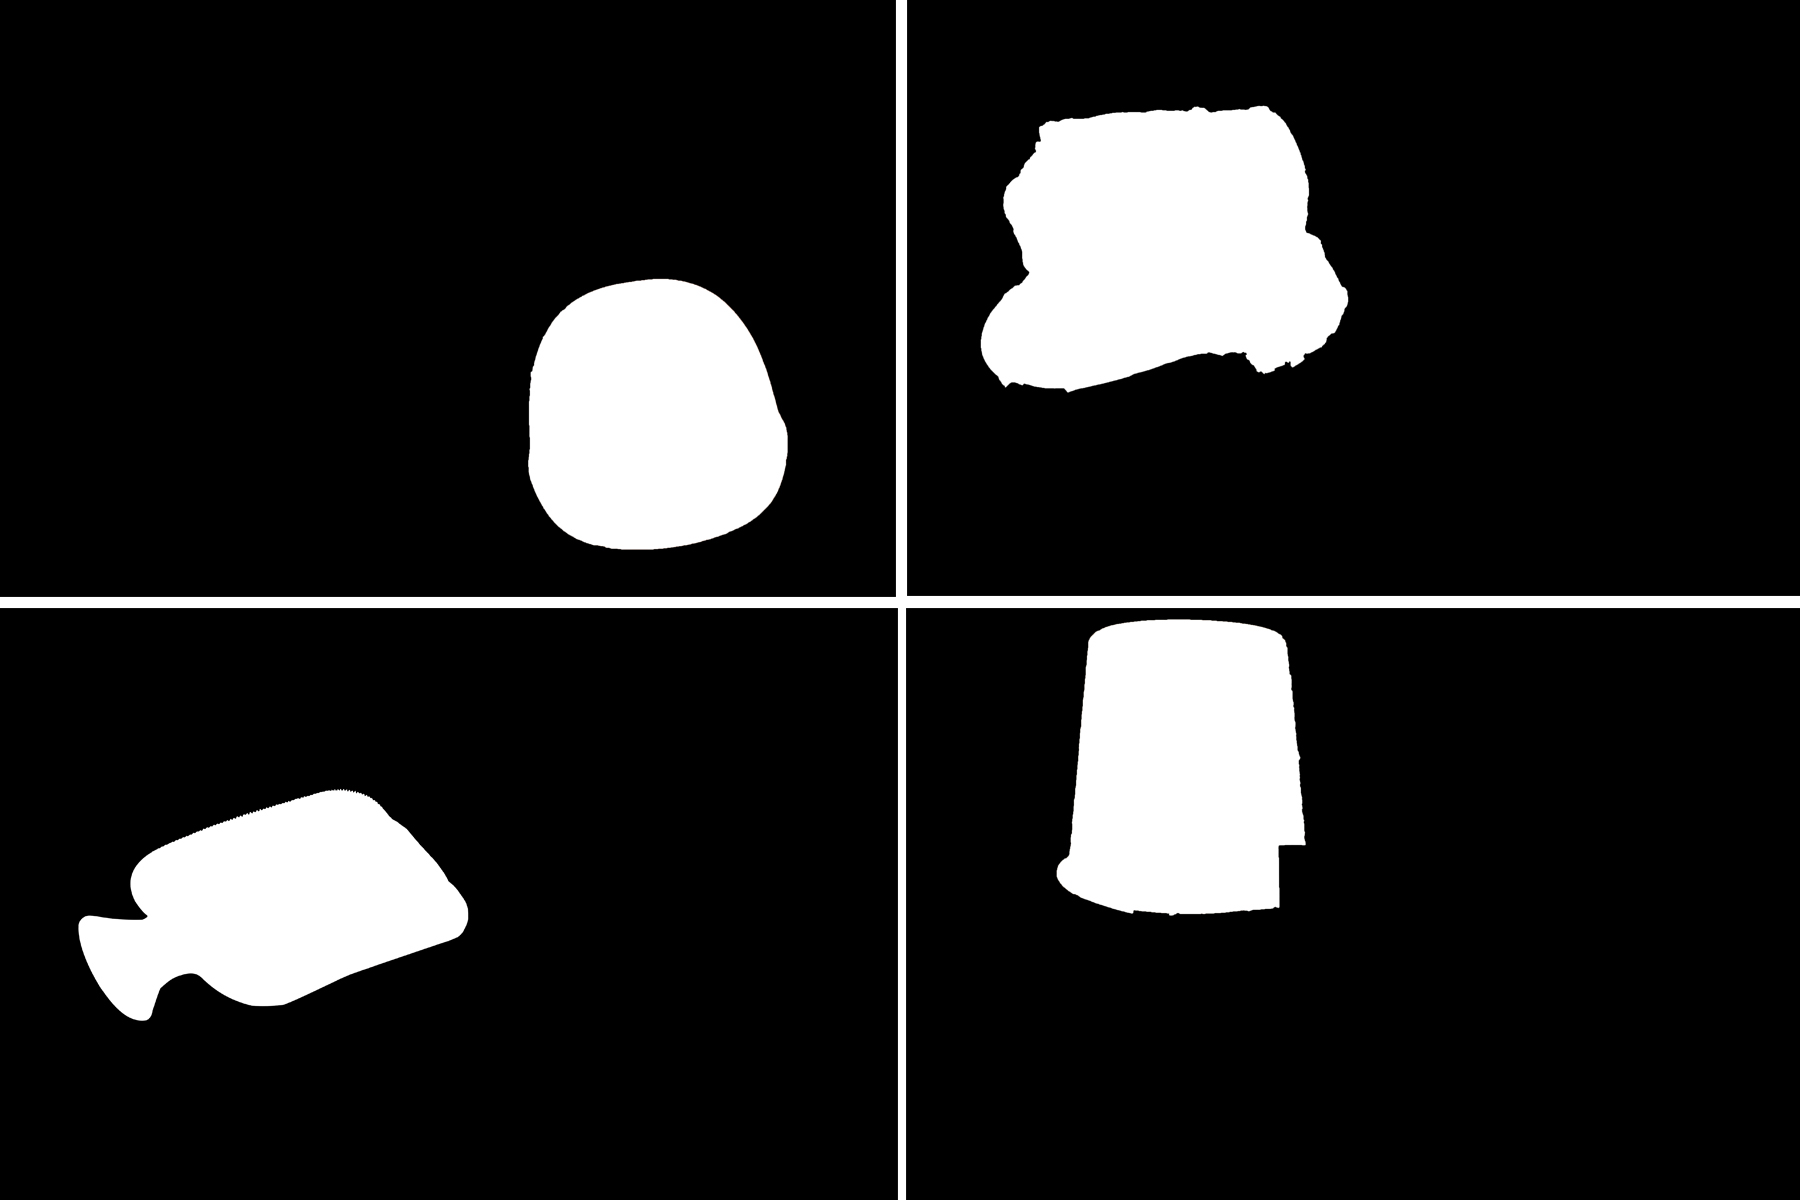
\includegraphics[width=12cm]{Images/batch1_mask.jpg}			
	\caption[Bildunterschrift]{Bildunterschrift.}
	\label{fig:batch1mask}
\end{figure}

\begin{figure}[H] 
	\center 
	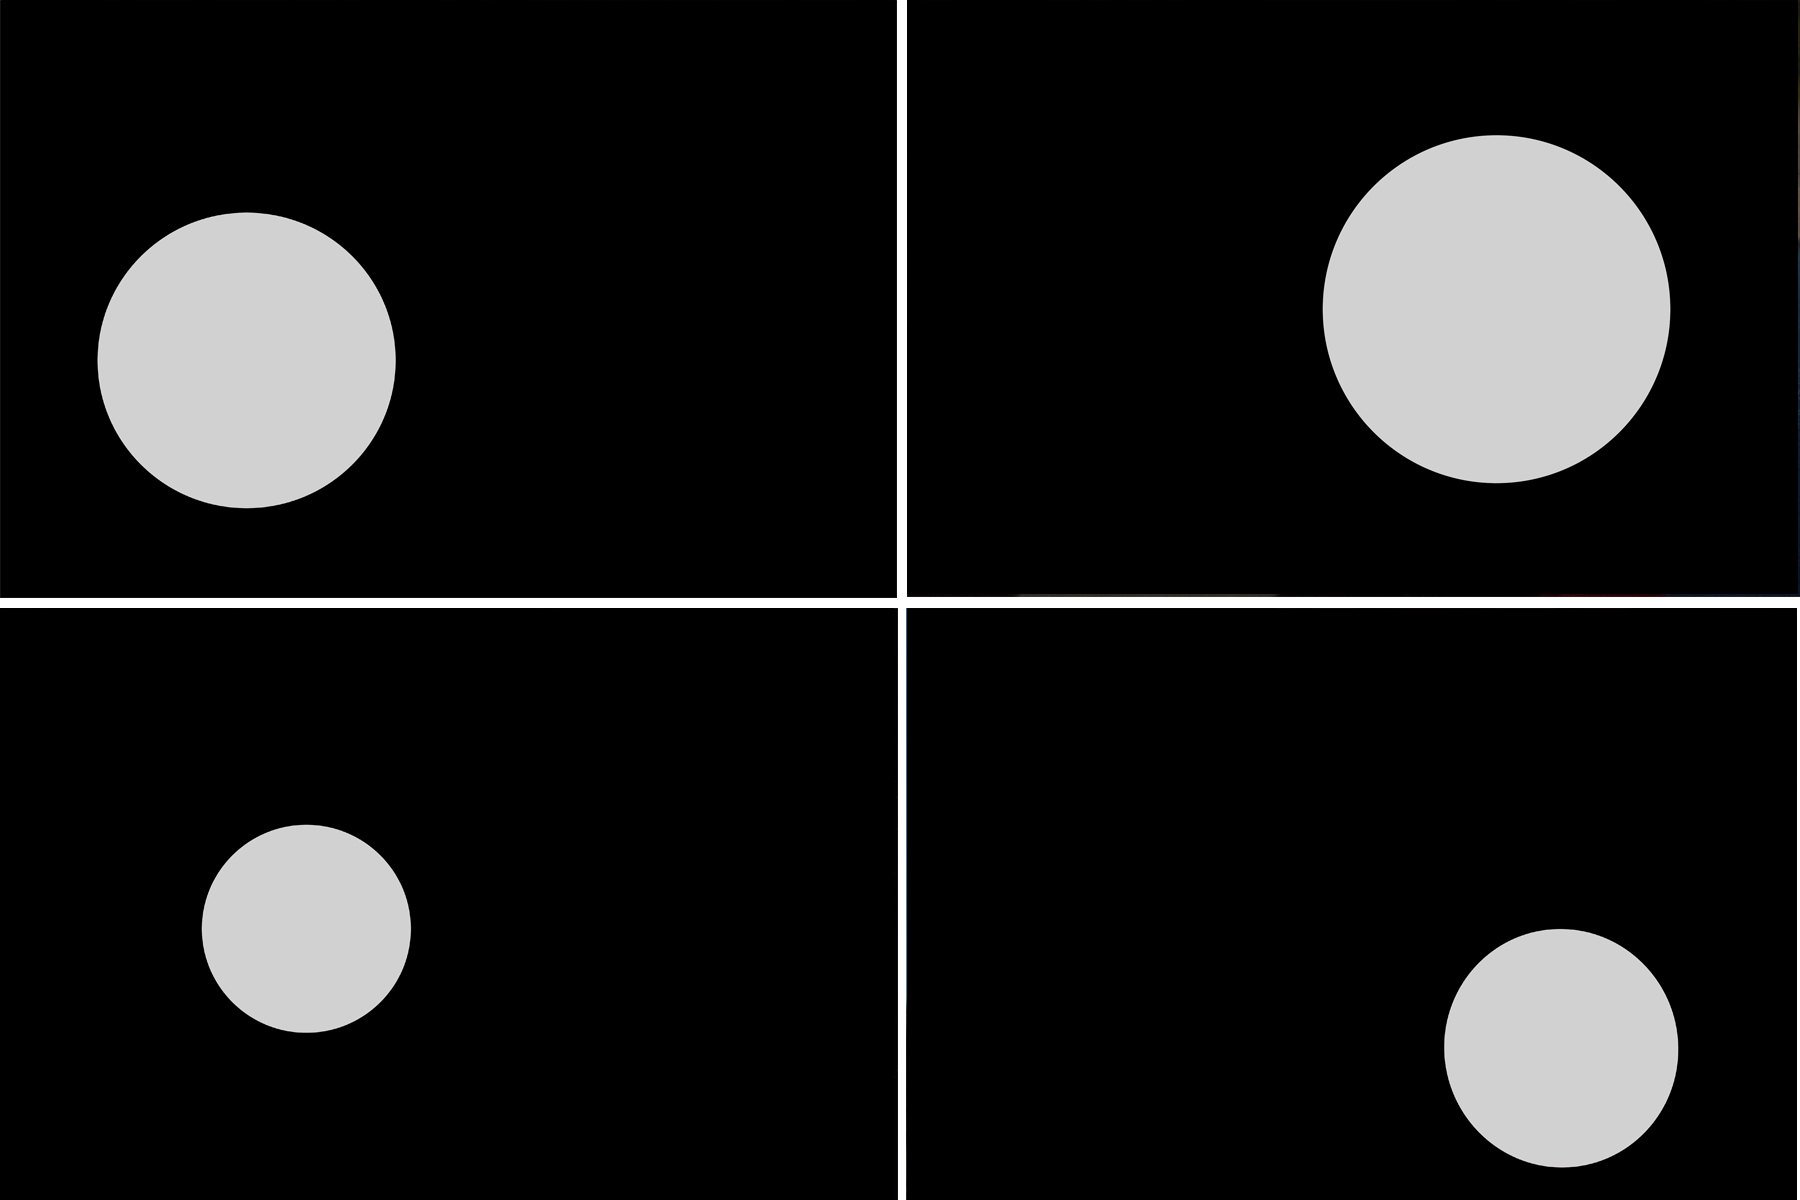
\includegraphics[width=12cm]{Images/batch2_mask.jpg}			
	\caption[Bildunterschrift]{Bildunterschrift.}
	\label{fig:batch2mask}
\end{figure}

\subsection{Subcontours}\label{sec:subcontours}
\todo[inline, color=red]{Vera}

\subsection{Different Approaches}\label{sec:approaches}
\todo[inline, color=yellow]{Laura}
Because no reliable solution could be found, three different approaches were tried out. 
All three approaches are based on the paper of Johnson and Farid \cite{Johnson}. 
Whereas two of this approaches remained unchanged (compare section~\ref{sec:appOne} and \ref{sec:appTwo}), the last approach takes the assumptions of Johnson and Farid and expand them (compare section~\ref{sec:appThree}). \\
To standardise the explanations in the following sections a list of necessary variables is introduced: 
\begin{itemize}
\item $\vec{L}$: vector, which points in the direction of the light source (3D)
\item $\vec{N}(x,y)$: surface normal at the point (x,y) (3D)
\item $I(x,y)$: intensity at the point (x,y)
\item $A$: constant ambient light term
\item $R$: constant reflectance value
\end{itemize}
All equations in this section, as well as its subsections, are taken from \cite{Johnson}. The basic idea behind the approach of Johnson and Farid is summed up in equation \ref{equ:General}.

\begin{equation}
\label{equ:General}
I(x,y) = R(\vec{N}(x,y)\cdot \vec{L}) + A
\end{equation}

In the following sections we do not have a three dimensional room, as all evaluations are made based on images. All of them have in common, that their assumptions are based on a infinite light source in a two dimensional image space. Therefore $\vec{L}$ and $\vec{N}(x,y)$ needs to be redefined as follows:
\begin{itemize}
\item $\vec{L}$: vector, which points in the direction of the light source (2D)
\item $\vec{N}(x,y)$: surface normal at the point (x,y) (2D)
\end{itemize}

For the second and the third approach, the light vectors are summed up in patches of size four. 

\subsubsection{1. Approach: One Lightvector}\label{sec:appOne}
\todo[inline, color=yellow]{Laura}
The first approach tries to simplify the two dimensional case by solving equation \ref{equ:firstApp} and getting one finale light vector per contour of an object plus the ambient light term. The Matrix $M$ can be found in Johnsons and Farids paper \cite{Johnson} in equation (6) and $p$ denotes the number of points on a contour with the same assumed reflectance. All other variables are explained in section~\ref{sec:approaches}. Thereby the reflectance along the entire contour is thought of as constant. 

\begin{equation}
\label{equ:firstApp}
E(\vec{L} , A) = 
\left\vert \left\vert 
M
\begin{pmatrix}
L_{x} \\
L_{y} \\
A \\
\end{pmatrix} -
\begin{pmatrix}
I(x_{1} , y_{1}) \\
I(x_{2} , y_{2}) \\
\vdots \\
I(x_{p} , y_{p}) \\
\end{pmatrix}
 \right\vert\right\vert^{2}
 = \left\vert \left\vert  M\vec{v}-\vec{b}  \right\vert\right\vert^{2}
\end{equation}

This options can be activated in our script \textit{mainwindow.cpp} by setting \textit{usePatches} to \textit{false}. Equation~\ref{equ:firstApp} is than solved using \textit{Singular Value Decomposition}. Then the lightvector $\vec{L}$ is drawn onto the test image to visualize the result.  

\subsubsection{2. Approach: Averaging Lightvectors}\label{sec:appTwo}
\todo[inline, color=yellow]{Laura}
For the second approach it is not only assumed, that the light source is infinite, but also that the reflection created by it is constant within each surface patch. The basic idea can be found in section 2.2.1 in the paper of Johnson and Farid \cite{Johnson}.\\
It is assumed, that a minimization problem according to equation~\ref{equ:secondApp} needs to be solved. The Matrix $M$ can be found in \cite{Johnson} in equation (8). \\

\begin{equation}
\label{equ:secondApp}
E_{1}(\vec{L}^{\,1} , ... , \vec{L}^{\,n} , A) = 
\left\vert \left\vert 
M
\begin{pmatrix}
L^{1}_{x} \\
L^{1}_{y} \\
\vdots  \\
L^{n}_{x} \\
L^{n}_{y} \\
A \\
\end{pmatrix} -
\begin{pmatrix}
I(x^{1}_{1} , y^{1}_{1}) \\
\vdots  \\
I(x^{1}_{p} , y^{1}_{p}) \\
\vdots  \\
I(x^{n}_{1} , y^{n}_{1}) \\
\vdots  \\
I(x^{n}_{p} , y^{n}_{p}) \\
\end{pmatrix}
 \right\vert\right\vert^{2}
 = \left\vert \left\vert  M\vec{v}-\vec{b}  \right\vert\right\vert^{2}
\end{equation}
This options can be activated in our script \textit{mainwindow.cpp} by setting \textit{usePatches} to \textit{true} and \textit{useHighestIntensity} to \textit{false}.
As stated in section~\ref{sec:appOne} equation~\ref{equ:secondApp} is solved using \textit{Singular Value Decomposition} as well. This leads to calculating one light vector per patch. To get the final vector $\vec{L}$ all of this light vectors are averaged.


\subsubsection{3. Approach: Lightvector with highest Intensity}\label{sec:appThree}
\todo[inline, color=red]{Laura}
This last approach uses the same basic idea as the second one described in section \ref{equ:secondApp}. It is also based on dividing the surface normals $\vec{N}$ into patches and solving equation~\ref{equ:secondApp} using \textit{Singular Value Decomposition}. Afterwards there is no averaging done, but the vector $\vec{L}$ belonging to the patch with the highest intensities is taken as the final light vector. \\
This idea is not described in the paper of Johnson and Farid~\cite{Johnson}. It was a try make the results of the \textit{Lighting Detector} more trustworthy. \\
This options can be activated in our script \textit{mainwindow.cpp} by setting \textit{usePatches} to \textit{true} and \textit{useHighestIntensity} to \textit{true}.

\newpage